\documentclass[tikz,border=14pt]{standalone}
\usepackage{amsmath}
\usetikzlibrary{arrows.meta,positioning}
\definecolor{ink}{HTML}{243449}
\definecolor{teal}{HTML}{087F8C}
\definecolor{violet}{HTML}{7354B5}
\begin{document}
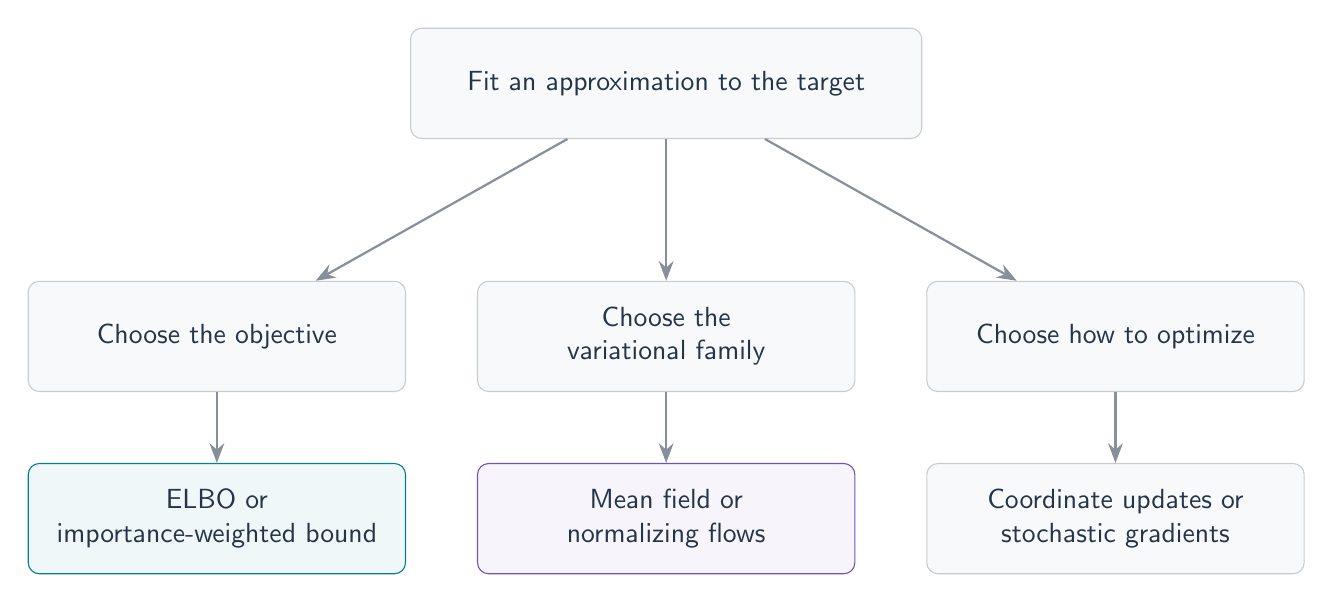
\begin{tikzpicture}[font=\sffamily,node distance=9mm and 9mm,
box/.style={draw=ink!25,rounded corners=4pt,fill=ink!3,text=ink,align=center,text width=43mm,minimum height=14mm,inner sep=7pt},
edge/.style={-{Stealth[length=2.5mm]},thick,draw=ink!55}]
\node[box,text width=60mm] (a) {Fit an approximation to the target};
\node[box,below=18mm of a] (c) {Choose the\\variational family};
\node[box,left=of c] (b) {Choose the objective};
\node[box,right=of c] (d) {Choose how to optimize};
\node[box,below=of b,draw=teal,fill=teal!6] (e) {ELBO or\\importance-weighted bound};
\node[box,below=of c,draw=violet,fill=violet!6] (f) {Mean field or\\normalizing flows};
\node[box,below=of d] (g) {Coordinate updates or\\stochastic gradients};
\foreach \s/\t in {a/b,a/c,a/d,b/e,c/f,d/g}\draw[edge] (\s)--(\t);
\end{tikzpicture}
\end{document}
